
\documentclass{article}

\usepackage{amssymb} %chekmark symbol
\usepackage{graphicx}

\begin{document}

\date{versie 22 maart 2015}
\title{low-level scenario FR-P003}
\maketitle


%%%%%%%%%%%% BIBLIOTHEKEN
\subsubsection*{BIBLIOTHEKEN}
\vspace{2 mm}

\textbf{ID}: FR-P003
\vspace{2 mm}

\begin{figure}[!h]
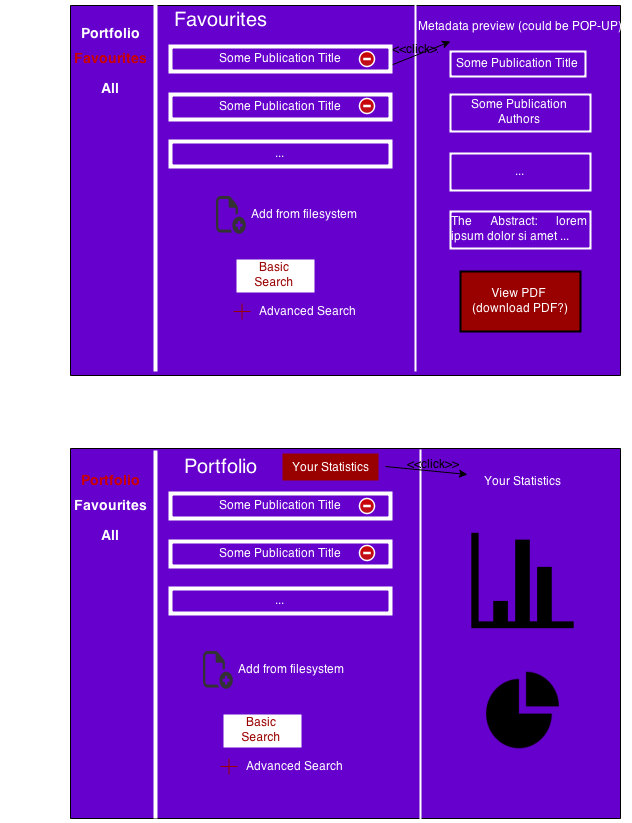
\includegraphics[width=1.1\textwidth]{library.png}
\caption{Wireframe functionaliteiten library. Bovenste figuur geldt voor alle drie de bibliotheken, onderstaande figuur beschrijft de extra "statistieken" functionaliteit (NOG NIET ONTWIKKELD) voor portfolio's.  }
\end{figure}


\hrule
\vspace{2 mm}
\noindent \textbf{Scenario}:
\begin{description}
\item CLIENT : publicatie toevoegen (zie FR-P001), publicatie opzoeken (zie FR-P002) en publicaties verwijderen of van bibliotheek veranderen (zie server API). Opmerkingen:
	\begin{description}
	\item Wanneer een gebruiker na een basic search een publicatie wil toevoegen die gevonden is via google scholar, moet hetzelfde proces om metadata manueel aan te vullen (beschreven in FR-P001) doorlopen worden. Hou er dus rekening mee in de GUI dat de "publicatie toevoegen" functionaliteit meerdere keren kan opduiken 
	\item "your statistics" is nog niet ge�mplementeerd, maar moet dus uiteindelijk wel in het design van de portfolio bibliotheek zitten.
	 \end{description}
 \end{description}
 \noindent wireframe zie volgende pagina.



\end{document}





